\documentclass[10pt,aspectratio=169]{beamer}

\usetheme{metropolis}

\usepackage{booktabs}
\usepackage{pgfplots}
\usepackage{listings}
\usepackage{xcolor}

\lstset{
	basicstyle=\ttfamily,
	frame=shadowbox,
	rulesepcolor=\color{gray},
	columns=fullflexible,
	commentstyle=\color{gray},
	keywordstyle=\bfseries\color{red},
	escapeinside={\%*}{*)},
  aboveskip=2em,
  captionpos=b,
  abovecaptionskip=1em,
  belowcaptionskip=1em
}

\title{Midway presentation}
\subtitle{Group 1}
\date{12 November 2018}
\author{Claudio Maggioni}
\titlegraphic{\centering{
\includegraphics[height=1cm]{logo.png}}}

\begin{document}

\maketitle

\begin{frame}[standout]
\centering{\Huge Slides in \LaTeX}
\end{frame}

\section{What we've done so far}


\begin{frame}[fragile]{Search box}
\vfill\centering{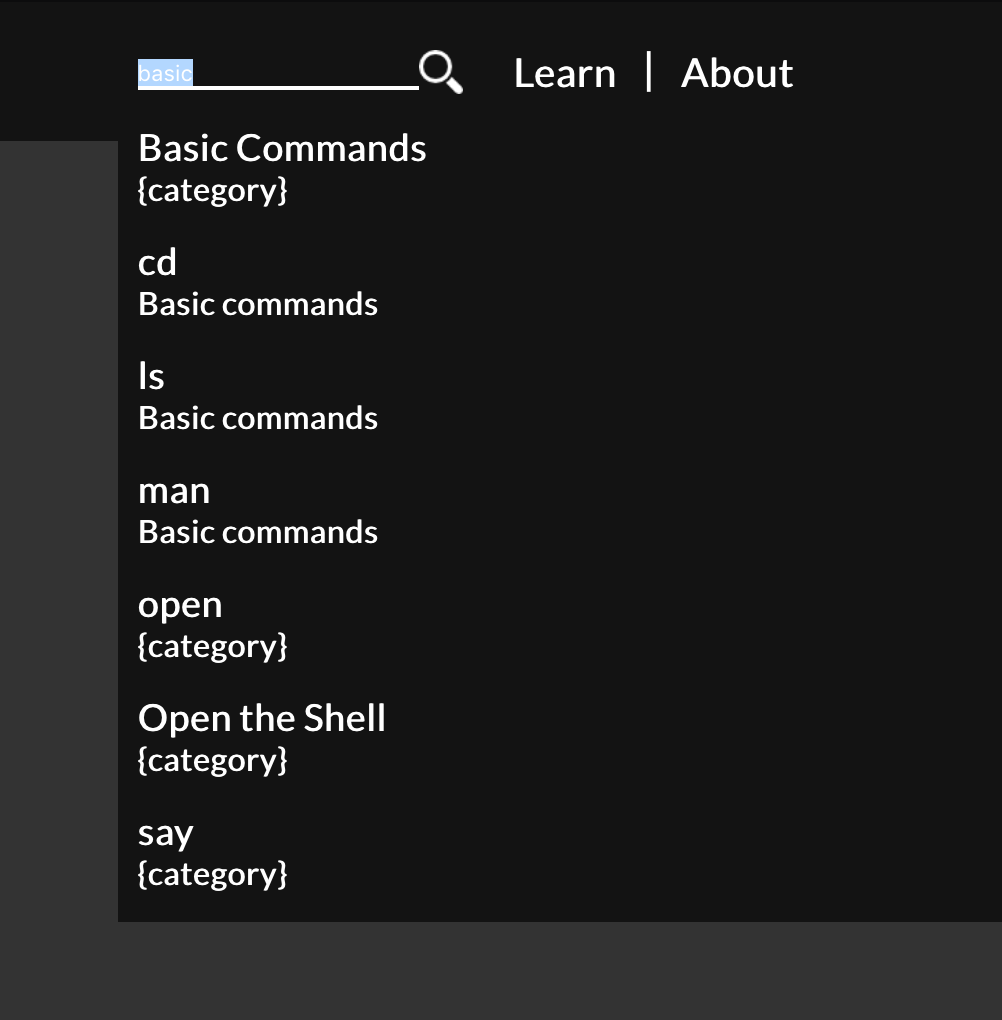
\includegraphics[width=0.7\textwidth]{search.png}}\vfill
\end{frame}


\begin{frame}[fragile]{Automatic topic index pages}
\vfill\centering{
\includegraphics[width=0.7\textwidth]{index.png}}\vfill
\end{frame}


\begin{frame}[fragile]{Basic style}
\vfill\centering{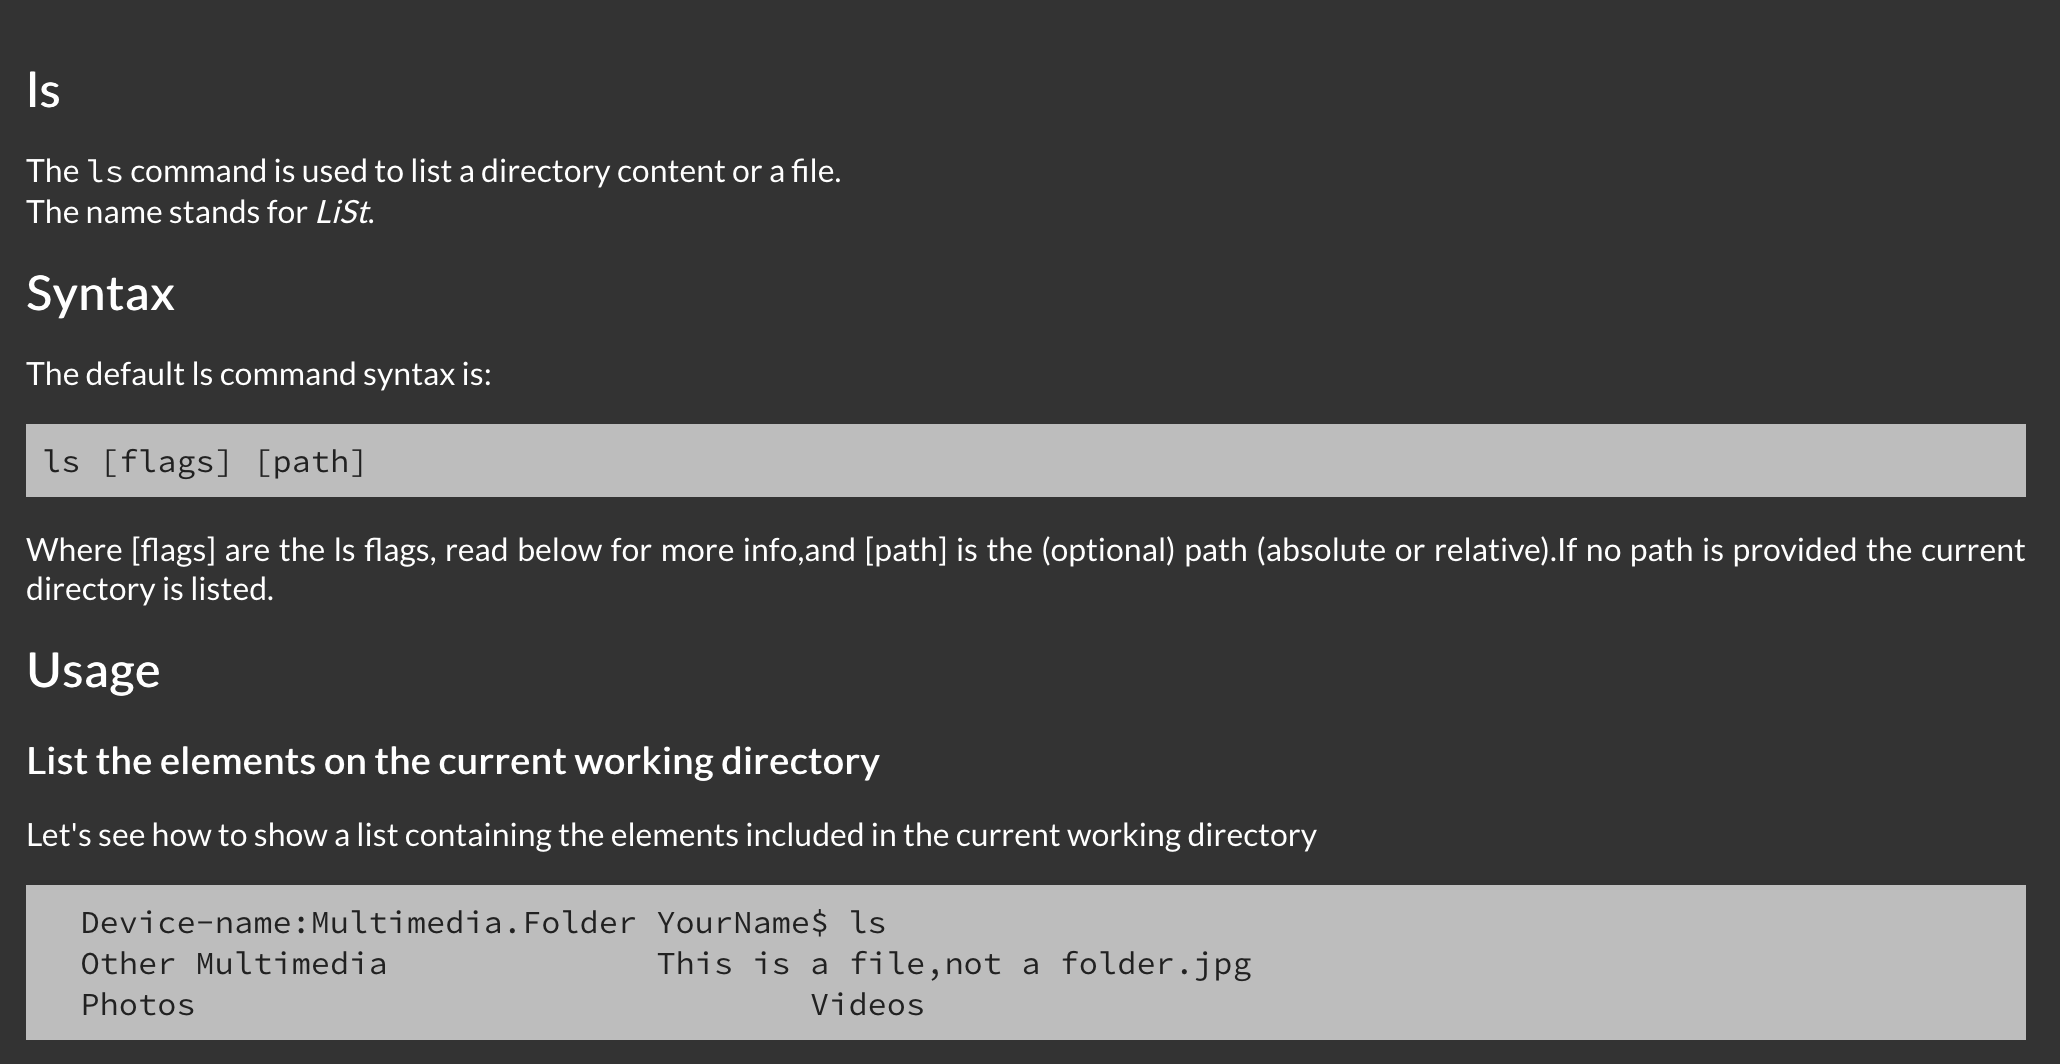
\includegraphics[width=0.8\textwidth]{formatting.png}}\vfill
\end{frame}


\begin{frame}[fragile]{Automatic attribution (in footer)}
\vfill\centering{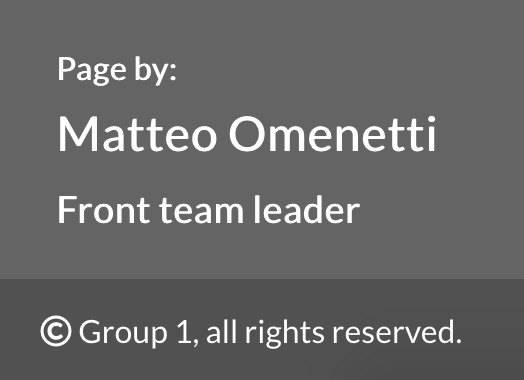
\includegraphics[width=0.7\textwidth]{footer.png}}\vfill
\end{frame}


\begin{frame}[fragile]{Automatic attribution (in about page)}
\vfill\centering{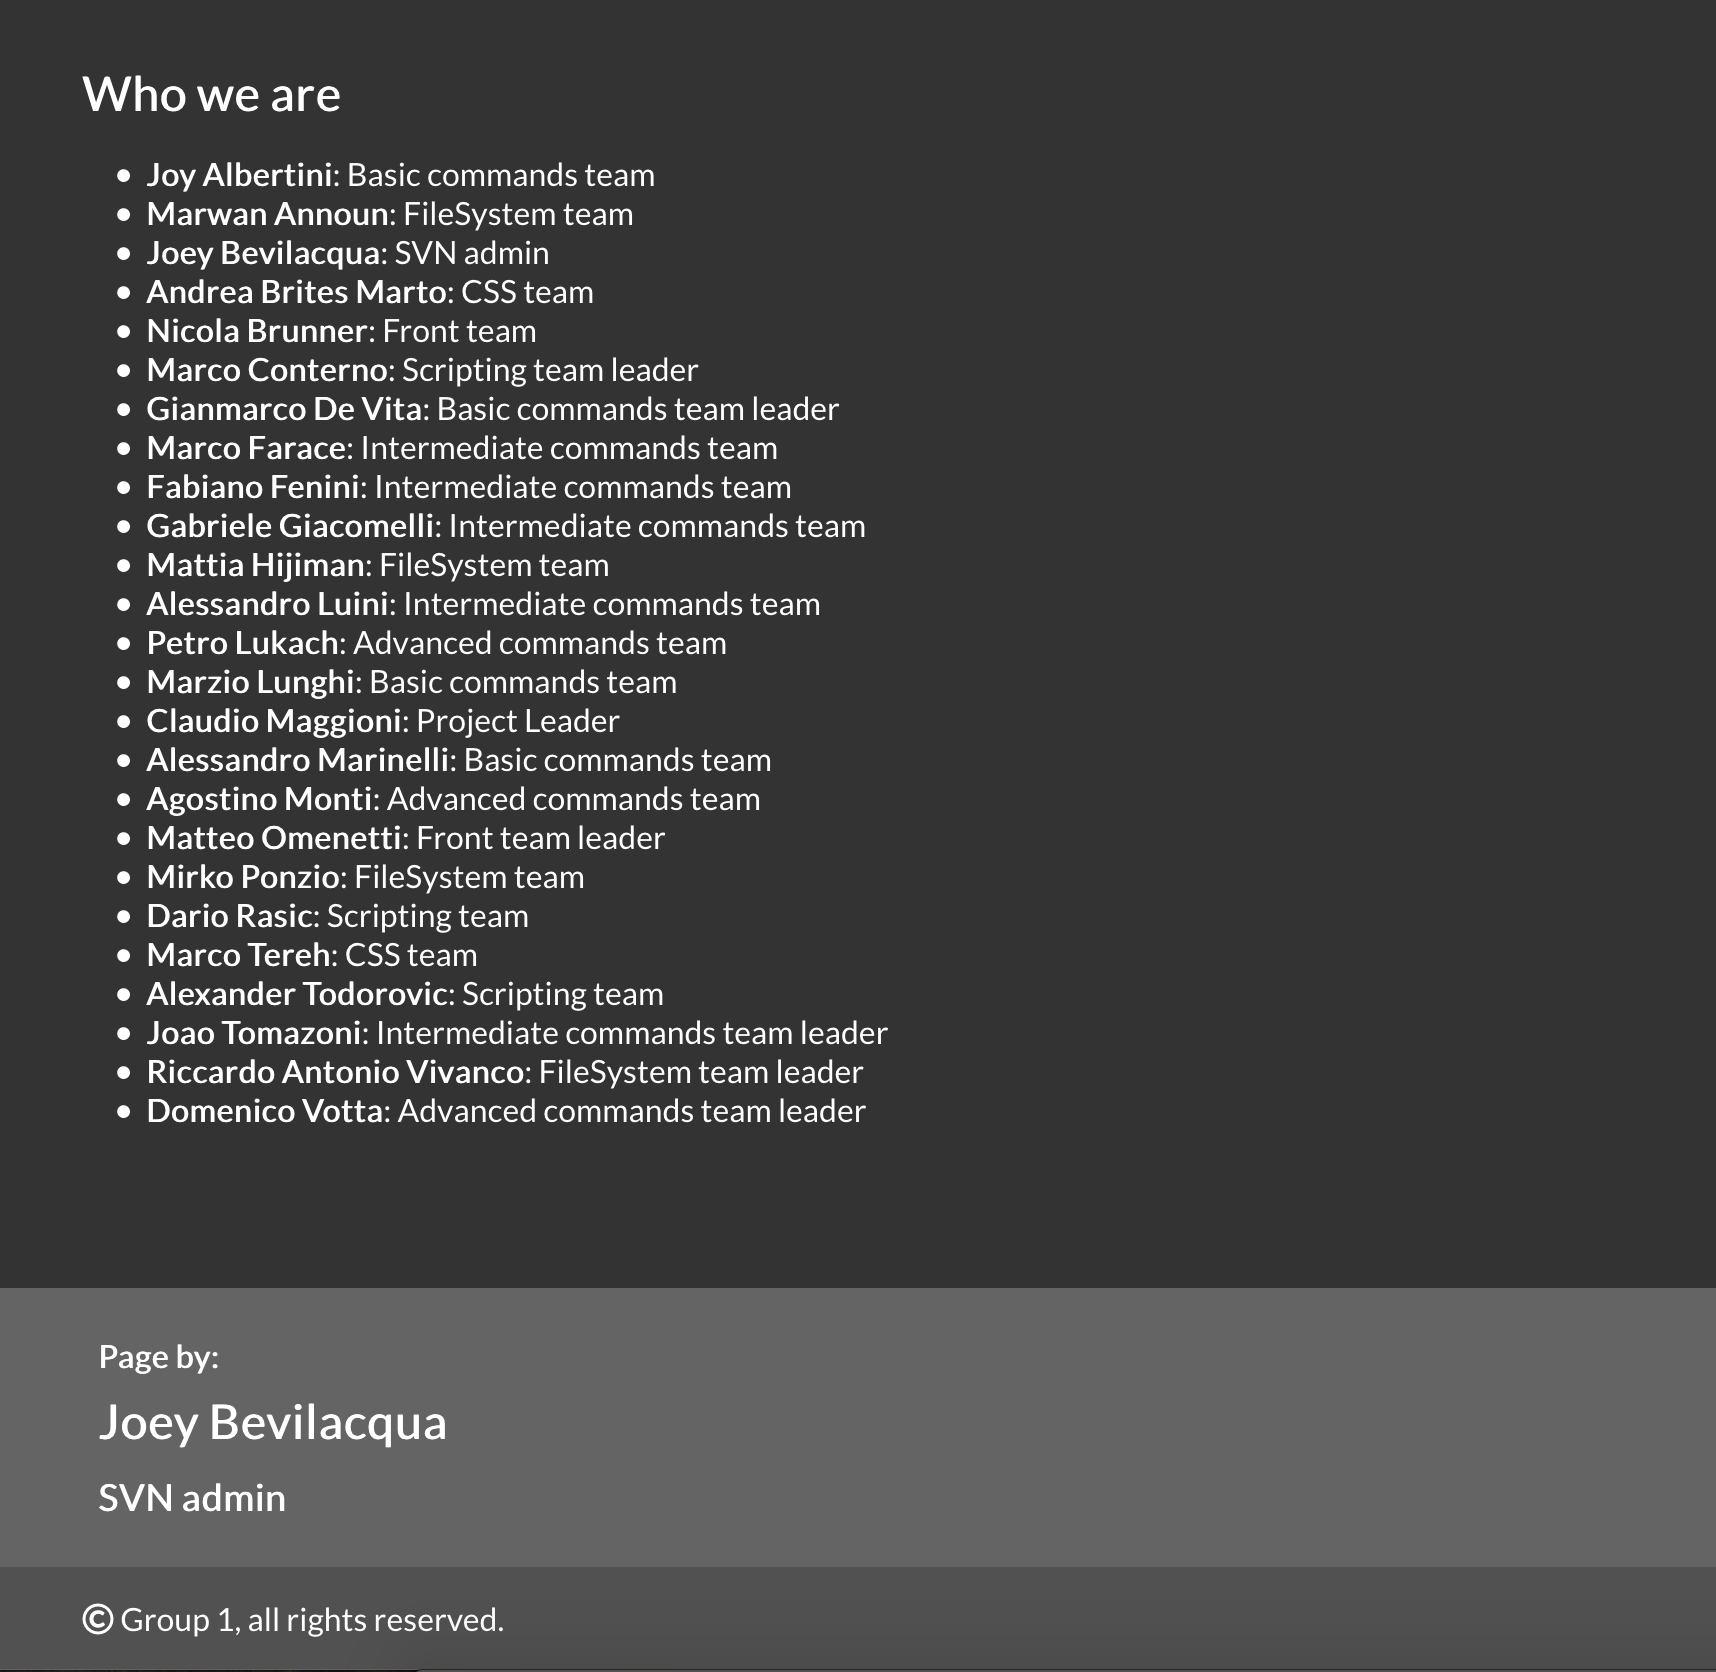
\includegraphics[width=0.7\textwidth]{about.png}}\vfill
\end{frame}


\begin{frame}[fragile]{Bonus 1 almost done}
\vfill\centering{
\includegraphics[width=0.45\textwidth]{rust.png}}\vfill
\end{frame}


\begin{frame}[standout]
\centering{\Huge Nystrom seal of quality}
\end{frame}


\section{First code review for content}

{\setbeamercolor{background canvas}{bg=black}
\begin{frame}
\centering{\Huge\ttfamily\color{green} 
	\textsc{From HTML \\
	to Jekyll\\
	\vspace{0.5cm}
	\Large was not that easy \ldots}}
\end{frame}}


\begin{frame}[fragile]{From this \ldots}
\begin{figure}[h]
\begin{lstlisting}[language=html]
<html>
<head>
    <meta author="Fabiano Fenini" />
    ...
</head>
<body>
<header>
    <h1>cat</h1>
    ...
</header>
...
</body>
</html>
\end{lstlisting}
\end{figure}
\end{frame}


\begin{frame}[fragile]{\ldots to this}
\begin{figure}[h]
\begin{lstlisting}[language=html]
---
layout: page
category-page: intermediate
category-title: Intermediate commands
tags: cat content file show concatenate
author: Fabiano Fenini
title: cat
---

<p>
...
</p>
\end{lstlisting}
\end{figure}
\end{frame}


\begin{frame}{Page creation guide}
\vfill\centering{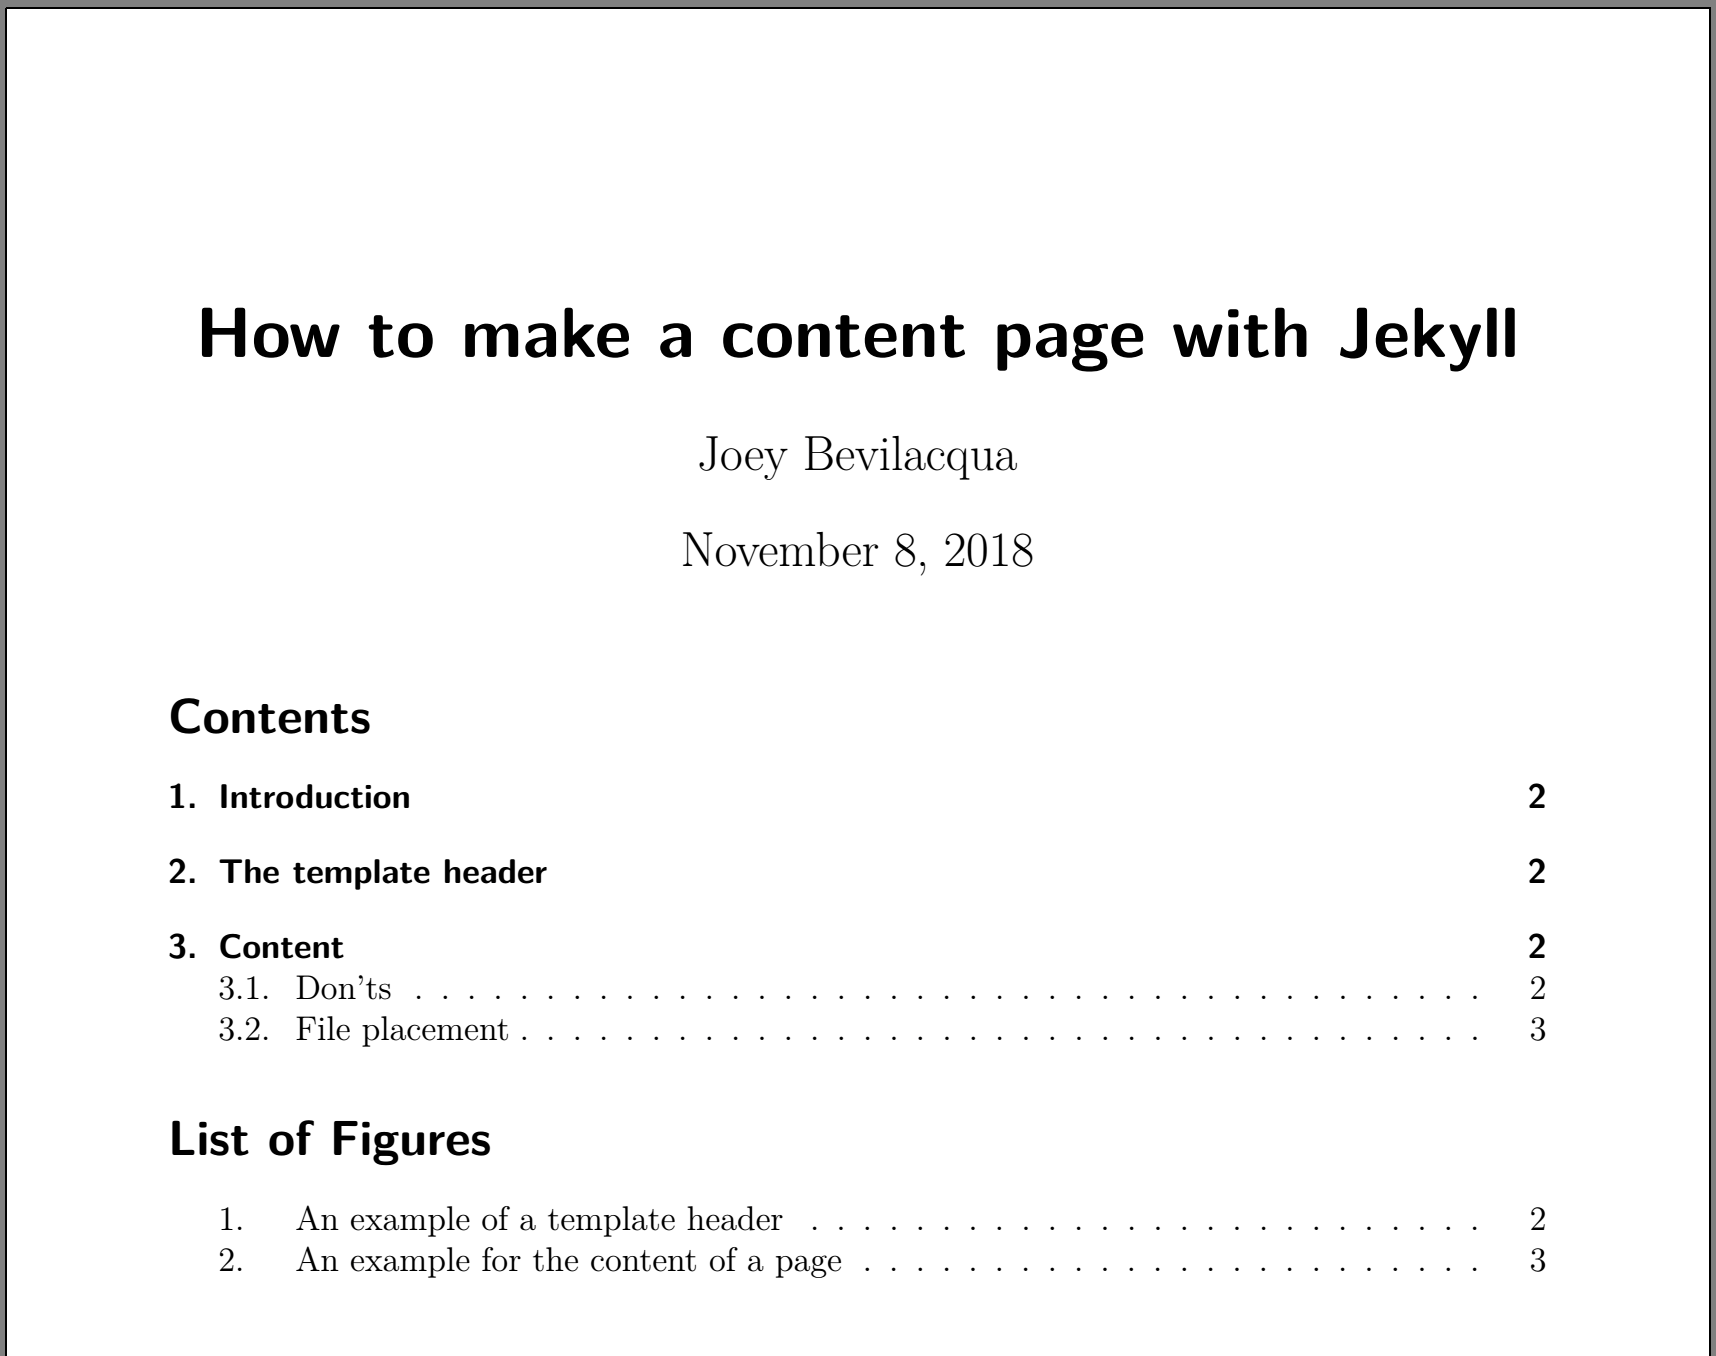
\includegraphics[width=0.6\textwidth]{page_creation.png}}\vfill
\end{frame}


\begin{frame}{The Jekyll header}
\begin{table}[h]
\begin{tabular}{l l}
\textbf{Variable} & \textbf{Use} \\
layout & Template for the page\\
category-page & Automatic topic pages creation\\
category-title & Indexing in search\\
tags & Keywords for search\\
author & Automatic content attribution\\
title & Title of the page\\
\end{tabular}
\end{table}
\end{frame}


\begin{frame}[standout]
\centering{\Huge Demo time!}
\end{frame}

\end{document}
